\documentclass{standalone}
\usepackage{tikz}
\usetikzlibrary{patterns, positioning}

\begin{document}
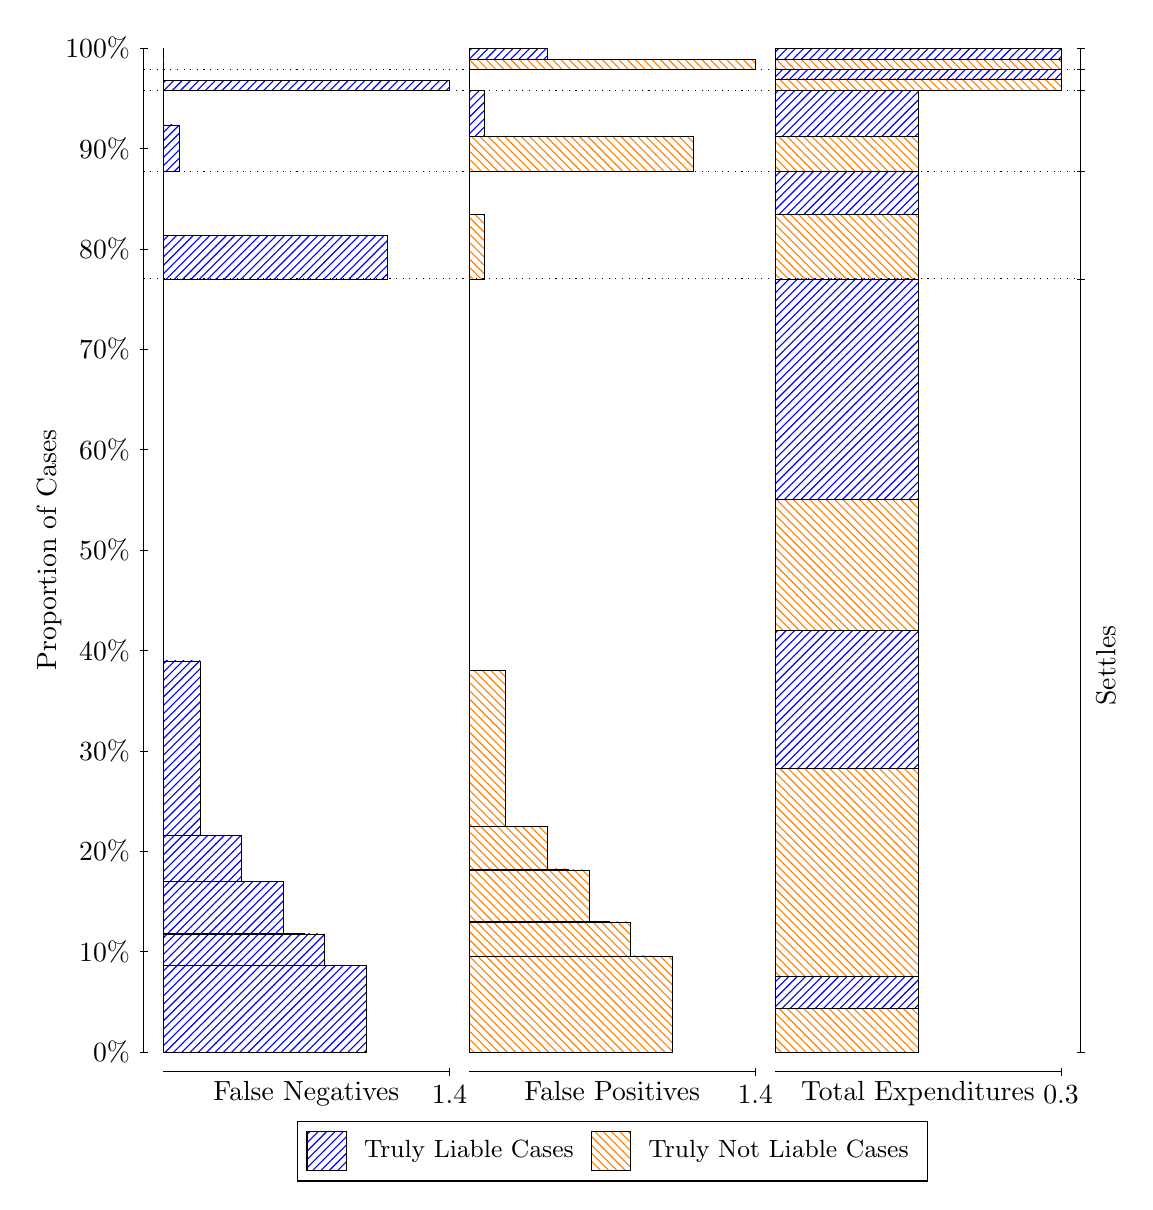
\begin{tikzpicture}
\draw[black, very thin] (1.5,1.75) -- (1.5,14.5);
\node[rotate=90, anchor=center] at (0.3, 8.125) {Proportion of Cases};
\draw[black, very thin] (1.45,1.75) -- (1.55,1.75);
\node[anchor=east] at (1.45, 1.75) {0\%};
\draw[black, very thin] (1.45,3.025) -- (1.55,3.025);
\node[anchor=east] at (1.45, 3.025) {10\%};
\draw[black, very thin] (1.45,4.3) -- (1.55,4.3);
\node[anchor=east] at (1.45, 4.3) {20\%};
\draw[black, very thin] (1.45,5.575) -- (1.55,5.575);
\node[anchor=east] at (1.45, 5.575) {30\%};
\draw[black, very thin] (1.45,6.85) -- (1.55,6.85);
\node[anchor=east] at (1.45, 6.85) {40\%};
\draw[black, very thin] (1.45,8.125) -- (1.55,8.125);
\node[anchor=east] at (1.45, 8.125) {50\%};
\draw[black, very thin] (1.45,9.4) -- (1.55,9.4);
\node[anchor=east] at (1.45, 9.4) {60\%};
\draw[black, very thin] (1.45,10.675) -- (1.55,10.675);
\node[anchor=east] at (1.45, 10.675) {70\%};
\draw[black, very thin] (1.45,11.95) -- (1.55,11.95);
\node[anchor=east] at (1.45, 11.95) {80\%};
\draw[black, very thin] (1.45,13.225) -- (1.55,13.225);
\node[anchor=east] at (1.45, 13.225) {90\%};
\draw[black, very thin] (1.45,14.5) -- (1.55,14.5);
\node[anchor=east] at (1.45, 14.5) {100\%};

\draw[black, very thin] (13.4,1.75) -- (13.4,14.5);
\draw[black, very thin] (13.35,1.75) -- (13.45,1.75);
\node[anchor=west] at (13.35, 1.75) {};
\draw[black, very thin] (13.35,11.568) -- (13.45,11.568);
\node[anchor=west] at (13.35, 11.568) {};
\draw[black, very thin] (13.35,12.935) -- (13.45,12.935);
\node[anchor=west] at (13.35, 12.935) {};
\draw[black, very thin] (13.35,13.963) -- (13.45,13.963);
\node[anchor=west] at (13.35, 13.963) {};
\draw[black, very thin] (13.35,14.231) -- (13.45,14.231);
\node[anchor=west] at (13.35, 14.231) {};
\draw[black, very thin] (13.35,14.5) -- (13.45,14.5);
\node[anchor=west] at (13.35, 14.5) {};

\draw[black, very thin, pattern color=blue, pattern=north east lines] (1.75,1.75) rectangle (4.3264,2.8489);
\draw[black, very thin, pattern color=blue, pattern=north east lines] (1.75,2.8489) rectangle (3.7979,3.2492);
\draw[black, very thin, pattern color=blue, pattern=north east lines] (1.75,3.2492) rectangle (3.5336,3.2559);
\draw[black, very thin, pattern color=blue, pattern=north east lines] (1.75,3.2559) rectangle (3.2694,3.9135);
\draw[black, very thin, pattern color=blue, pattern=north east lines] (1.75,3.9135) rectangle (3.0052,3.9161);
\draw[black, very thin, pattern color=blue, pattern=north east lines] (1.75,3.9161) rectangle (2.7409,4.501);
\draw[black, very thin, pattern color=blue, pattern=north east lines] (1.75,4.501) rectangle (2.4767,4.5037);
\draw[black, very thin, pattern color=blue, pattern=north east lines] (1.75,4.5037) rectangle (2.2124,6.7178);
\draw[black, very thin, pattern color=orange, pattern=north west lines] (1.75,6.7178) rectangle (1.75,11.568);
\draw[black, very thin, pattern color=blue, pattern=north east lines] (1.75,11.568) rectangle (4.5906,12.117);
\draw[black, very thin, pattern color=orange, pattern=north west lines] (1.75,12.117) rectangle (1.75,12.935);
\draw[black, very thin, pattern color=blue, pattern=north east lines] (1.75,12.935) rectangle (1.9482,13.524);
\draw[black, very thin, pattern color=orange, pattern=north west lines] (1.75,13.524) rectangle (1.75,13.963);
\draw[black, very thin, pattern color=blue, pattern=north east lines] (1.75,13.963) rectangle (5.3833,14.085);
\draw[black, very thin, pattern color=orange, pattern=north west lines] (1.75,14.085) rectangle (1.75,14.231);
\draw[black, very thin, pattern color=orange, pattern=north west lines] (1.75,14.231) rectangle (1.75,14.354);
\draw[black, very thin, pattern color=blue, pattern=north east lines] (1.75,14.354) rectangle (1.75,14.5);
\draw[black, very thin, pattern color=orange, pattern=north west lines] (5.6333,1.75) rectangle (8.2097,2.9666);
\draw[black, very thin, pattern color=orange, pattern=north west lines] (5.6333,2.9666) rectangle (7.9455,2.9699);
\draw[black, very thin, pattern color=orange, pattern=north west lines] (5.6333,2.9699) rectangle (7.6812,3.4011);
\draw[black, very thin, pattern color=orange, pattern=north west lines] (5.6333,3.4011) rectangle (7.417,3.4043);
\draw[black, very thin, pattern color=orange, pattern=north west lines] (5.6333,3.4043) rectangle (7.1527,4.0634);
\draw[black, very thin, pattern color=orange, pattern=north west lines] (5.6333,4.0634) rectangle (6.8885,4.0738);
\draw[black, very thin, pattern color=orange, pattern=north west lines] (5.6333,4.0738) rectangle (6.6242,4.6129);
\draw[black, very thin, pattern color=orange, pattern=north west lines] (5.6333,4.6129) rectangle (6.0958,6.5998);
\draw[black, very thin, pattern color=blue, pattern=north east lines] (5.6333,6.5998) rectangle (5.6333,11.568);
\draw[black, very thin, pattern color=orange, pattern=north west lines] (5.6333,11.568) rectangle (5.8315,12.385);
\draw[black, very thin, pattern color=blue, pattern=north east lines] (5.6333,12.385) rectangle (5.6333,12.935);
\draw[black, very thin, pattern color=orange, pattern=north west lines] (5.6333,12.935) rectangle (8.4739,13.374);
\draw[black, very thin, pattern color=blue, pattern=north east lines] (5.6333,13.374) rectangle (5.8315,13.963);
\draw[black, very thin, pattern color=orange, pattern=north west lines] (5.6333,13.963) rectangle (5.6333,14.109);
\draw[black, very thin, pattern color=blue, pattern=north east lines] (5.6333,14.109) rectangle (5.6333,14.231);
\draw[black, very thin, pattern color=orange, pattern=north west lines] (5.6333,14.231) rectangle (9.2667,14.354);
\draw[black, very thin, pattern color=blue, pattern=north east lines] (5.6333,14.354) rectangle (6.6242,14.5);
\draw[black, very thin, pattern color=orange, pattern=north west lines] (9.5167,1.75) rectangle (11.333,2.2995);
\draw[black, very thin, pattern color=blue, pattern=north east lines] (9.5167,2.2995) rectangle (11.333,2.7065);
\draw[black, very thin, pattern color=orange, pattern=north west lines] (9.5167,2.7065) rectangle (11.333,5.3526);
\draw[black, very thin, pattern color=blue, pattern=north east lines] (9.5167,5.3526) rectangle (11.333,7.109);
\draw[black, very thin, pattern color=orange, pattern=north west lines] (9.5167,7.109) rectangle (11.333,8.7633);
\draw[black, very thin, pattern color=blue, pattern=north east lines] (9.5167,8.7633) rectangle (11.333,11.568);
\draw[black, very thin, pattern color=orange, pattern=north west lines] (9.5167,11.568) rectangle (11.333,12.385);
\draw[black, very thin, pattern color=blue, pattern=north east lines] (9.5167,12.385) rectangle (11.333,12.935);
\draw[black, very thin, pattern color=orange, pattern=north west lines] (9.5167,12.935) rectangle (11.333,13.374);
\draw[black, very thin, pattern color=blue, pattern=north east lines] (9.5167,13.374) rectangle (11.333,13.963);
\draw[black, very thin, pattern color=orange, pattern=north west lines] (9.5167,13.963) rectangle (13.15,14.109);
\draw[black, very thin, pattern color=blue, pattern=north east lines] (9.5167,14.109) rectangle (13.15,14.231);
\draw[black, very thin, pattern color=orange, pattern=north west lines] (9.5167,14.231) rectangle (13.15,14.354);
\draw[black, very thin, pattern color=blue, pattern=north east lines] (9.5167,14.354) rectangle (13.15,14.5);
\draw[black, dotted] (1.5,11.568) -- (13.4,11.568);
\draw[black, dotted] (1.5,12.935) -- (13.4,12.935);
\draw[black, dotted] (1.5,13.963) -- (13.4,13.963);
\draw[black, dotted] (1.5,14.231) -- (13.4,14.231);
\draw[black, very thin] (1.75,1.5) -- (5.3833,1.5);
\node[anchor=north] at (3.5667, 1.5) {False Negatives};
\draw[black, very thin] (5.3833,1.45) -- (5.3833,1.55);
\node[anchor=north] at (5.3833, 1.45) {1.4};

\draw[black, very thin] (5.6333,1.5) -- (9.2667,1.5);
\node[anchor=north] at (7.45, 1.5) {False Positives};
\draw[black, very thin] (9.2667,1.45) -- (9.2667,1.55);
\node[anchor=north] at (9.2667, 1.45) {1.4};

\draw[black, very thin] (9.5167,1.5) -- (13.15,1.5);
\node[anchor=north] at (11.333, 1.5) {Total Expenditures};
\draw[black, very thin] (13.15,1.45) -- (13.15,1.55);
\node[anchor=north] at (13.15, 1.45) {0.3};

\node[black, centered, rotate=90] at (13.72, 6.6588) {Settles};





\draw (7.449999999999999,1.5) node[draw=none] (baseCoordinate) {};
\begin{scope}[align=center]
        \matrix[scale=0.5, draw=black, below=0.5cm of baseCoordinate, nodes={draw}, column sep=0.1cm]{
            \node[rectangle, draw, minimum width=0.5cm, minimum height=0.5cm, pattern=north east lines, pattern color=blue] {}; &
            \node[draw=none, font=\small] (B) {Truly Liable Cases}; &
            \node[rectangle, draw, minimum width=0.5cm, minimum height=0.5cm, pattern=north west lines, pattern color=orange] {}; &
            \node[draw=none, font=\small] (B) {Truly Not Liable Cases}; \\
            };
\end{scope}

\end{tikzpicture}
\end{document}